\chapter{Logica}
Un sistema logico formale è costituito da:
\begin{itemize}
    \item \textbf{Linguaggio}: sintassi (come sono formate le frasi) e semantica (come assegnare un significato ad una frase) e 
    pragmatica (come usare la logica per un obiettivo preciso)
    \item \textbf{Apparato d'inferenza}: permette di studiare le relazioni fra le frasi di un linguaggio 
\end{itemize}

\section{Logica Proposizionale}
Consiste nella logica delle proposizioni, in particolare associamo ad ogni proposizione un valore true o false.\smallskip\\
\colorbox{SALZO}{\parbox{\dimexpr\linewidth-2\fboxsep}{\begin{definition}
   L'\textbf{alfabeto proposizionale} è composto da:
   \begin{itemize}
    \item \textbf{Simboli non logici}: un insieme numerabile $\mathcal{P}$ di simboli chiamati \textit{varibili proposizionali} o \textit{atomi proposizionali} o 
   \textit{lettere proposizionali }
   \item \textbf{Simboli logici (Connettivi)}: $\{ \neg, \wedge,\vee,\to, \equiv \}$
   \item \textbf{Simboli separatori}: "(" e ")"
   \end{itemize} 
\end{definition}}}\smallskip\\
Il significato dei connettivi è il seguente:
   \begin{itemize}[label = --]
    \item $\bm{\neg}$: è il simbolo di \textbf{negazione}
    \item $\bm{\wedge}$: è il simbolo di \textbf{congiunzione}
    \item $\bm{\vee}$: è il simbolo di \textbf{disgiunzione} (o)
    \item $\bm{\to}$: è il simbolo di \textbf{implicazione}
    \item $\bm{\equiv}$: è il simbolo di \textbf{equivalenza}
   \end{itemize}
   Nello spiegare la logica proposizionale, spesso faremo riferimento a definizioni di insiemi e funzioni in maniera \textbf{induttivo}.
   Lavorare con l'induzione significa fornire uno o più passi base, seguiti dal passo induttivo.\smallskip\\
   \textit{Esempio.} L'insieme dei numeri naturali \textsc{nat} è definito induttivamente come segue:
   \begin{itemize}
    \item \textbf{Passo base}: $0 \in \textsc{nat}$
    \item \textbf{Passo induttivo}: se $x\in \textsc{nat}$ allora $s(x) \in \textsc{nat}$
   \end{itemize}
   Dove $s(x)$ è la funzione successore che associa ad ogni numero $x$ il suo successore $x +1$.\newpage
   \noindent Definiamo in maniera induttiva le \textbf{formule} (o frasi) \textbf{ben formate}\smallskip\\
\colorbox{SALZO}{\parbox{\dimexpr\linewidth-2\fboxsep}{\begin{definition}
   Una formula (frase) della logica proposizionale dell'alfabeto $\mathcal{P}$ è un espressione finita costruita secondo la seguente
   definizione induttiva:
   \begin{itemize}
    \item (passo base ?) Ogni $P \in \mathcal{P}$ è una \textit{formula atomica}, e ogni formula atomica è una formula,
    questo significa che ogni lettera proposizionale è una formula (che è atomica).
    \item Se $A$ e $B$ sono formule, allora anche le seguenti sono formule:
    \begin{itemize}
        \item (A)
        \item $\neg A$
        \item $A \wedge B$
        \item $A \vee B$
        \item $A \to B$
        \item $A \equiv B$
    \end{itemize}
   \end{itemize}
\end{definition}}}\smallskip\\
Ecco alcuni esempi di formule ben formate:
\[  P \to Q    \]
\[  P \to (P \to R)    \]
\[   P \wedge Q \to R   \]
Ecco invece alcuni esempi di non formule:
\[  PQ \qquad \text{non c'è alcun connettivo}    \]
\[  (P \to \wedge ((Q \to R)  \qquad \text{le parentesi non sono ben formate}  \]
\[   P \wedge Q \to \neg R \neg  \qquad \text{connettivi messi a cazzo}   \]
Ma quando non ci sono le parentesi, in che ordine dobbiamo calcolare le formule? \\Prendiamo ad esempio le seguenti formule:
\[     (P \wedge Q) \to R \qquad P\wedge (Q\to R)       \]
hanno gli stessi connettori, ma non sono assolutamente due formule equivalenti. Per risolvere il problema di come intendere l'ordine di una formula
esiste una \textbf{tabella della priorità}:
\begin{center}
\begin{tabular}{|c|c|}
    \hline
    Connettivo & Priorità \\
    \hline
    $\neg$ & 1 \\
    $\wedge$ & 2 \\
    $\vee$ & 3 \\
    $\to $ & 4 \\
    $\equiv$ & 5 \\
    \hline
\end{tabular}
\end{center}
Una formula può essere rappresentata come un \textbf{albero} dove le foglie sono associate ad una variabile proposizionale,
mentre gli altri nodi sono associati ai connettivi.\smallskip\\
\textit{Esempio.} Ecco l'albero della formula $(A \wedge \neg B)\equiv(B \to C)$
\begin{figure}[H]
    \centering  
    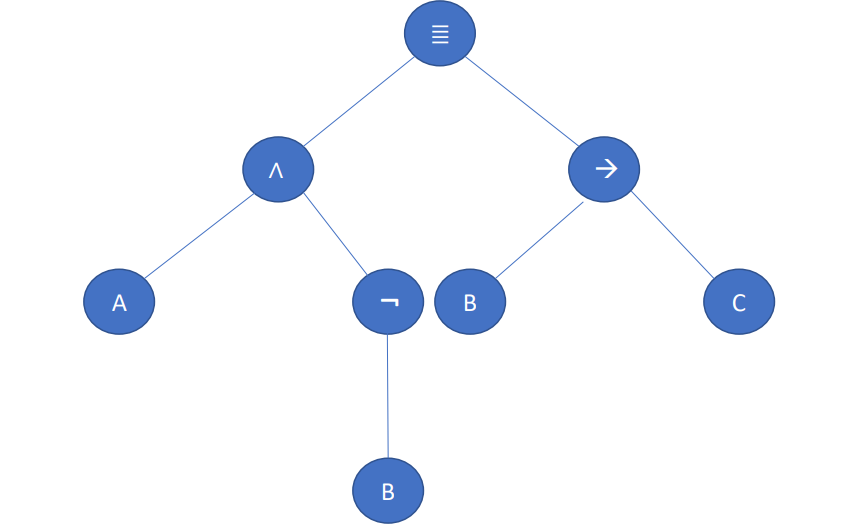
\includegraphics[width=0.6\linewidth]{../../images/albe.png}
    %\caption{caption}
    %\label{label}
\end{figure}
\noindent Dalla rappresentazione ad albero delle formule è chiaro che esitano delle \textbf{sottoformule}:
\begin{itemize}
    \item $A$ è una sottoformula di se stessa
    \item $A$ è una sottoformula di di $\neg A$, e $A$ è una sottoformula di $(A)$
    \item $A,B$ sono sottoformule di $A \wedge B, A\vee B, A \to B, A\equiv B$
    \item Se $A$ è una sottoformula di $B$ e $B$ è una sottoformula di $C$, allora $A$ è una sottoformula di $C$
    \item $A$ è una sottoformula "proper" di $B$ se $A$ è una sottoformula di $B$ e $A$ è diversa da $B$
\end{itemize}
Fino ad ora abbiamo visto il lessico, ora passiamo alla \textbf{semantica}. Si assegna ad ogni proposizione dell'alfabeto un
\textbf{valore di verità}. Per valutare la verdicità di una formula abbiamo bisogno di un \textbf{contesto}, infatti non posso vedere una formula e 
dire a priori se è vera o falsa. Ad esempio la proposizione "Oggi piove" non possiamo dire se è vera o falsa senza un contesto,
ma dobbiamo sapere se è sta effettivamente piovendo o no.\smallskip\\
\colorbox{SALZO}{\parbox{\dimexpr\linewidth-2\fboxsep}{\begin{definition}
   Dato un certo alfabeto proposizionale con lettere proposizionali $\mathcal{P}$, una \textbf{interpretazione logica proposizionale} è una funzione che assegna ad ogni lettera 
   dell'alfabeto \textit{true} o \textit{false}, ovvero:
   \[  \mathcal{I} : \mathcal{P} \to \{ \text{True, False}\}  \]
\end{definition}}}\smallskip\\
Non si può dire se una formula è vera o falsa senza un \textbf{contesto}, che nella logica proposizionale si dice \textbf{interpretazione logico proposizionale}.
Esiste un contesto (interpretazione) in cui non posso dire nè true nè false? Assolutamente no, in logica proposizionale
è \textbf{sempre} possibile dire se una formula è vera o falsa. Esistono delle formule che possono essere valutate true o false 
per qualunque interpretazione possibile. Ad esempio:
\[   A \wedge \neg A  \]
è sempre falsa per qualunque interpretazione possibile.\\
Inoltre per convenzione indicheremo con $P$ la lettera proposizionale per cui il valore di verità è true, formalmente:
\[\mathcal{I} = \{ P \in \mathcal{P} \ | \ \mathcal{I}(P) = \text{True}    \}\]
Ora definiamo induttivamente la \textbf{valutazione} di una formula all'interno di una \textbf{interpretazione}:\smallskip\\
\colorbox{SALZO}{\parbox{\dimexpr\linewidth-2\fboxsep}{\begin{definition}
   $\mathcal{I} \bm{\models A}$ è definita induttivamente come segue:
   \begin{itemize}
    \item Se $A$ è una lettera proposizionale $P$, cioè se $P \in \mathcal{P}$, allora $\mathcal{I}\models A$ se e solo se
    \[  \mathcal{I}(P) = \text{True}   \]
    \item $\mathcal{I}\models A$ se e solo se $\models A$
    \item $\mathcal{I}\models A$ se e solo se non è il caso in cui $\mathcal{I}\models A$ (possiamo scrivere $\not\models A$)
    \item $\mathcal{I}\models A \wedge B$ se e solo se valgono entrambi $\mathcal{I}\models A$ e $\mathcal{I}\models B$ 
    \item $\mathcal{I}\models A \vee B$ se e solo se vale $\mathcal{I}\models A$ oppure $\mathcal{I}\models B$
    \item $\mathcal{I}\models A\to B$ se solo se non è il caso in cui $\mathcal{I}\models A$ e $\mathcal{I} \not\models A$
    \item $\mathcal{I}\models A\equiv B$ se e solo se valgono sia $\mathcal{I}\models A\to B$ sia $\mathcal{I}\models B \to A$
   \end{itemize}
\end{definition}}}\smallskip\\
Quindi, possiamo leggere $\mathcal{I} \models A$ come se fosse:
\[  \text{L'interpretazione } \mathcal{I} \text{ soddisfa la formula } A   \]
Vediamo un esempio di come arrivare alla valutazione di una formula:\smallskip\\
\textit{Esempio.} Consideriamo l'interpretazione $\mathcal{I} = \{ P  \}$, e valutiamo l'interpretazione $\mathcal{I} \models (P \wedge Q) \vee (R \to S) $.\\
Ricordiamo che quando un interpretazione è rappresentata da un insieme, le lettere presenti nell'insieme sono vere (true), le altre no.
In questo caso allora $P$ è true, mentre $Q,R$ e $S$ sono false. Per valutare l'interpretazione, facciamo le valutazioni delle singole formule, rispettando l'ordine di priorità:
\[   \underbrace{(\text{True } \wedge \text{ False})}_{\text{False}}  \vee \underbrace{(\text{False }\to \text{ False})}_{\text{True}}   \]
\[ \text{False } \vee \text{ True}  \]
\[   \boxed{\text{True}} \] 
Ora vediamo degli algoritmi  per valutare il valore di verità di una formula:  




 
Ecco alcune osservazioni sui connettivi nella logica proposizionale:
\begin{itemize}
    \item $A \to B$ ha lo stesso significato di $\neg A \vee B$
    \item $\neg (A\vee B)$ ha lo stesso significato di $\neg A \wedge \neg B$ (1 legge di De Morgan)
    \item $\neg (A \wedge B)$ ha lo stesso significato di $\neg A \vee \neg B$ (2 legge di De Morgan)
    \item $A \to B$ ha lo stesso significato di $\neg B \to \neg A$ (Contronominale?)
    \item $A \to \neg B$ ha lo stesso significato di $B \to \neg A$
    \item $A$ è una condizione sufficiente per $B$, si può scrivere $A \to B$ e si legge "se $A$ allora $B$"
    \item $A$ è una condizione necessaria per $B$, si può scrivere $B \to A$
    \item $A$ è una condizione necessaria e sufficiente per $B$, si può scrivere $A \equiv B$ e si legge "$A$ se e solo se $B$"
    \item \textbf{NAND} è un connettivo derivante dai connettivi $\neg$ e $\wedge$. $A$ NAND $B$ è definito come $\neg(A \wedge B)$
    \item \textbf{NOR} è un connettivo derivante dai connettivi $\neg $ e $\vee$. $A$ NOR $B$ è definito come $\neg(A \vee B)$ 
\end{itemize}
Due formule hanno lo stesso significato se per ogni interpretazione hanno lo stesso valore di verità. Tutte le formule 
della logica proposizionale si possono scrivere con una serie di NOT ($\neg$) oppure una serie di AND ($\wedge$).\smallskip\\
In base a queste osservazioni possiamo costruire dei semplici \textbf{algoritmi} per la valutazione di formule:
    \begin{verbatim}
        (A is p)                        check(I |= p):
                                            if I(p) = true
                                                then return YES
                                            else return NO

        (A is B /\ C)                   check(I |= B /\ C):
                                            if check(I |= B)
                                                then return check(I |= C)
                                            else return NO

        (A is B \/ C)                   check(I |= B \/ C):
                                            if check(I |= B)
                                                then return YES
                                            else return check(I |= C)

        (A is B -> C)                   check(I |= B -> C):
                                            if check(I |= B)
                                                then return check(I |= C)
                                            else return YES

        (A is B === C)                  check(I |= B === C):
                                            if check(I |= B)
                                                then return check(I |= C)
                                            else return not(check(I |= C))

        (A is (B))                      check(I |= (B)):
                                            return(I |= B)
\end{verbatim}
Osserviamo che il \textbf{costo} computazionale degli algoritmi per la valutazione di una formula  è \textbf{lineare}, poichè analizzo ogni nodo
dell'albero (riferito alla formula in esame) una sola volta.

\subsubsection{Esericizi}
Vediamo un esercizio sulla logica proposizionale (simile a quello che potrebbe essere il primo esercizio di esame):\smallskip\\
$\bullet$ Consideriamo un linguaggio proposizionale in cui $p$ significa "Paola è felice", $q$ significa "Paola dipinge" e $r$
significa "Renzo è felice". Formalizza le seguenti frasi:
\begin{enumerate}
    \item \textit{se Paola è felice e dipinge allora Renzo non è felice}
    \item \textit{se Paola è felice, allora dipinge}
    \item \textit{Paola è felice solo se dipinge}
\end{enumerate}
Le soluzioni sono:
\begin{enumerate}
    \item $p \wedge q \to r$  $\big(\{p,q,r \not\models f\}, \ \{ p,q \models f\}\big)$
    \item $p \to q$
    \item $\neg(p \wedge \neg A)$ oppure $\neg q \to \neg p$ oppure $p \to q$, sono tutte formule equivalenti
\end{enumerate}


\noindent $\bullet$ Consideriamo un linguaggio proposizionale in cui $r$ significa "\textit{rigore nei conti pubblici}", 
$e$ significa "\textit{sviluppo dell'economia}", $s$ significa "\textit{stagnazione}" e $f$ significa "\textit{spesa facile}". 
Formalizza le seguenti frasi: 

\begin{enumerate}
    \item \textit{il rigore nei conti pubblici contraddice lo sviluppo economico} 
    \item \textit{se c'è stagnazione, allora non c'è sviluppo economico} 
    \item \textit{se c'è sviluppo economico, allora non c'è stagnazione} 
    \item \textit{la spesa facile è il contrario del rigore nei conti pubblici} 
\end{enumerate}
Le soluzioni sono:
\begin{enumerate}
    \item $r  \to\neg e$
    \item $s \to \neg e$
    \item $e \to \neg s$
    \item $f \equiv \neg r$
\end{enumerate}









